%% Based on a TeXnicCenter-Template by Tino Weinkauf.
%%%%%%%%%%%%%%%%%%%%%%%%%%%%%%%%%%%%%%%%%%%%%%%%%%%%%%%%%%%%%

%%%%%%%%%%%%%%%%%%%%%%%%%%%%%%%%%%%%%%%%%%%%%%%%%%%%%%%%%%%%%
%% HEADER
%%%%%%%%%%%%%%%%%%%%%%%%%%%%%%%%%%%%%%%%%%%%%%%%%%%%%%%%%%%%%
\documentclass[a4paper,twoside,10pt,twocolumn]{article}
% Alternative Options:
%	Paper Size: a4paper / a5paper / b5paper / letterpaper / legalpaper / executivepaper
% Duplex: oneside / twoside
% Base Font Size: 10pt / 11pt / 12pt

\setlength{\columnsep}{.25in}
% don't hyphenate so much - default = 200, max (never hyphenate) = 10,000
\hyphenpenalty=800
%\usepackage[francais]{babel}
\usepackage[T1]{fontenc}
\usepackage[latin1]{inputenc}

\usepackage[dvips]{graphicx} %%graphics and normal LaTeX


%% Math Packages %%%%%%%%%%%%%%%%%%%%%%%%%%%%%%%%%%%%%%%%%%%%
\usepackage{amsmath}
\usepackage{amsthm}
\usepackage{amsfonts}

\usepackage[square, comma, sort&compress]{natbib}
%% Line Spacing %%%%%%%%%%%%%%%%%%%%%%%%%%%%%%%%%%%%%%%%%%%%%
\usepackage{setspace}
\singlespacing        %% 1-spacing (default)
%\onehalfspacing       %% 1,5-spacing
%\doublespacing        %% 2-spacing


%% Other Packages %%%%%%%%%%%%%%%%%%%%%%%%%%%%%%%%%%%%%%%%%%%
\usepackage{a4wide} %%Smaller margins = more text per page.
%\usepackage{fancyhdr} %%Fancy headings
%\usepackage{longtable} %%For tables, that exceed one page
\usepackage{subfigure}


%
%%%%%%%%%%%%%%%%%%%%%%%%%%%%%%%%%%%%%%%%%%%%%%%%%%%%%%%%%%%%%

%%%%%%%%%%%%%%%%%%%%%%%%%%%%%%%%%%%%%%%%%%%%%%%%%%%%%%%%%%%%%
%% Options / Modifications
%%%%%%%%%%%%%%%%%%%%%%%%%%%%%%%%%%%%%%%%%%%%%%%%%%%%%%%%%%%%%

%\input{options} %You need a file 'options.tex' for this
%% ==> TeXnicCenter supplies some possible option files
%% ==> with its templates (File | New from Template...).



%%%%%%%%%%%%%%%%%%%%%%%%%%%%%%%%%%%%%%%%%%%%%%%%%%%%%%%%%%%%%
%% DOCUMENT
%%%%%%%%%%%%%%%%%%%%%%%%%%%%%%%%%%%%%%%%%%%%%%%%%%%%%%%%%%%%%
\begin{document}


\pagestyle{empty} %No headings for the first pages.


%% Title Page %%%%%%%%%%%%%%%%%%%%%%%%%%%%%%%%%%%%%%%%%%%%%%%
%% ==> Write your text here or include other files.

%% The simple version:
\title{Stochastic Search for a Target on a Textured Background}
\author{Alasdair D. F. Clarke, P. R. Green and M. J. Chantler}
%\date{} %%If commented, the current date is used.


\maketitle
\begin{abstract}
We present a comparison between human search performance and that of a stochastic model. The model uses the results of a Signal-Detection experiment to model target detectability and makes random saccades, weighted by empirically derived saccade amplitude and direction distributions. We compare the model against human performance in terms of the number of saccades required to find the target and the spatial distribution of the fixations. We find that the model compares well with human performance despite not integrating information across successive fixations or holding previously fixated image regions in any form of memory. 
\end{abstract}


%% The nice version:
%\input{titlepage} %%You need a file 'titlepage.tex' for this.
%% ==> TeXnicCenter supplies a possible titlepage file
%% ==> with its templates (File | New from Template...).

\pagestyle{plain} %Now display headings: headings / fancy / ...


%% Paper %%%%%%%%%%%%%%%%%%%%%%%%%%%%%%%%%%%%%%%%%%%%%%%%%

\section{Introduction}

Visual search is a common task which we encounter daily in real life. Within the confines of the laboratory search tasks frequently involve searching within an image for a designated target item. A complete computational model of visual search should contain two parts: a \itshape feature extraction mechanism \normalfont and a \itshape search strategy\normalfont. The feature extraction stage takes information from the stimulus and processes it in order to produce an activation map. This process should take both top-down guided search \citep{wolfe2007, zelinsky2008} and bottom-up saliency effects \citep{itti-koch2000, gao2008, itti-baldi2009} into account. For the sets of abstract, discrete search items commonly used as visual search stimuli, categorical features such as colour, orientation, shape and size are often used. Simple qualitative comparisons between the search items and the target are can be used to model top-down guidance \citep{pomplun2003, rutishauser-koch2007}. For more complex stimuli, such as a target hidden in image noise or in a photograph of a natural scene, we no longer have a discrete set of items to consider and  more sophisticated image processing techniques are required \citep{rao2002, zelinsky2008, pomplun2007,  hwang2009, tavassoli2009}.

\par

This study, however, is concerned with search strategies: the part of a model that uses an activation map to generate successive saccades. While a number of different mechanisms have been put forward, the most commonly implemented has been the maximum a priori (MAP) Observer. This strategy simply directs saccades to the current maximum of the activation map. A simple inhibition of return (IOR) mechanism is used to stop the model returning to previously fixated maxima and depending on the model, a maximum will either represent a search item, or the centre of gravity of a number of search items. As most previous computational models have primarily been interested in the feature extraction stage of search, this strategy has often been used for simplicity \citep{itti-koch2000, rao2002, pomplun2003, rutishauser-koch2007, clarke2009, zelinsky2008}.
 
\par

An alternative to the MAP Observer is the Ideal Observer which \cite{najemnik-geisler2005, najemnik-geisler2008} have derived for a search task involving a target hidden in $1/f$-noise. Their model is based on visibility maps calculated from empirical data collected during a signal detection experiment. These maps are used to control how much noise is added to potential target locations (with more noise at higher eccentricities) in the simulations. The Ideal Observer then makes saccades to the target location that will maximise the likelihood of it being able to identify the target during the following fixation. This contrasts with strategies where the model makes a saccade to the location which is currently most likely to be the target. In a second experiment observers carried out a prolonged search using similar stimuli. The results showed that over a range of task difficulties human observers take a similar number of saccades to the Ideal Observer. Furthermore, when averaged over all trials the Ideal Observer matched the spatial distribution of fixations: both the model and human observers exhibited a preference for fixating above and below the centre of the image. 
\par
Models like these are examples of systematic search. Broadly, systematic search can be made up from two types of behaviour. Firstly, the search could be controlled by image properties, in either a bottom-up or top-down manner, or a combination of both. Both the Guided Search \citep{wolfe2007} and saliency \citep{itti-koch2000} models fall into this category. Secondly, search strategies can also involve some serial dependence between one fixation and the next. This can include both memory processes (for example, inhibition of return) and regular scanning. However, some models, such as Rutishauser and Koch's probabilistic model [\citeyear{rutishauser-koch2007}] introduce a random element. The aim of this paper is to investigate whether, in a particular type of search task, an entirely random model of saccade selection can account for empirically recorded scan paths.

\par
Several general tendencies observed in scan-paths have been taken to be indicative of systematic search strategies. \cite{gilchrist-harvey2006} argue that the presence of horizontal bias in saccade directions indicates a systematic component in visual search and suggest that systematic tendencies can be hard to detect in scan-paths because of the interaction with salience-based object selection. Similarly, \cite{over2007} have shown that search scan-paths exhibit coarse-to-fine structures, i.e. observers make shorter saccades as a trial progresses. \cite{over2003} found that saccade directions are influenced by the edges of the search image and reported a preference for making saccades parallel to the boundaries of the stimuli. 
\par
Aks et al have argued that the presence of  $1/f$ dynamics in saccade-time series is evidence of a systematic component in visual search that relies on memory of previous fixation locations \citep{aks2002, aks2005}. They carried out the same time-series analysis on a random walk and found that it did not exhibit the same properties. However it is possible that Aks' result is an artefact of studying the compound time-series of large number of visual searches, one after another. If we were to look at the saccade amplitude time-series of several individual searches, each with a coarse-to-fine dynamic, then we would expect to see a strong low frequency component which could, at least partially, explain Aks et al.'s result. Similarly, \itshape distance-to-target \normalfont dynamics have been put forwards as evidence for some systematic component in visual search \citep{tseng-li2004}. These dynamics suggest that there are two phases to the search process: an ineffective stage, followed by an effective stage in which the distance from the current fixation location to the target decreases monotonically. However Greene has shown that these dynamics also arise in simple random walk simulations \citep{greene2008}. These simulations generated saccades at random and the target was assumed to be detected if it was within 20 pixels of the current fixation, and the model was given a maximum of 15 saccades to find the target. Further support for the idea of unsystematic visual search comes from several studies which show that memory only plays a small role in visual search tasks \citep{horowitz-wolfe1998, horowitz-wolfe2001, kuna2008, wolfe2000}. 
\par
Chance has been demonstrated to play a significant role in visual search performance. Using saccade amplitude distributions \cite{motter-holsapple2001} calculated the probability of fixating on the target by chance under different conditions. While this chance component decreases as the number of distracters increase, it continues to account for a sizeable fraction of performance. Random walks have been successfully used to model an observer's speed and accuracy in present/absent forced choice experiments \citep{stone1960, reeves2005}. Rather than model the spatial distribution of fixations these models simulate the observer's decision making process. The random walk occurs between two boundaries one for a target present response and one for target absent, and is governed by a drift and bias. 
\par
Overall, while there is strong evidence for systematic search in many tasks, the random element is stronger than we might expect in many others. However there is no clear evidence yet for purely random-walk search. In this paper we investigate just this, and ask if there are situations and stimuli for which a random-walk is a good model for human observers. A good place to look for such behaviour would be with simple stimuli (to avoid high-level semantic information from being used) containing a difficult to find target, such as a target embedded in noise. We have chosen to use fractal surfaces, which when illuminated give the appearance of a naturalistic surface texture \citep{clarke2008}. See Figure \ref{fig:smooth} for an example. These surfaces have two advantages over traditional visual search stimuli. Firstly, unlike the arrays of abstract discrete geometric objects that are often used, they appear naturalistic. Furthermore, unlike photographs of natural scenes, they are fully controlled and parametrised, and by controlling the seed of the random number generator many different, yet equivalent, textures can be created.
\par

\begin{figure}
	\centering
		
\includegraphics[width=\textwidth, bb=0 0 1024 1024]{figures/smooth512.png}
		\caption{An example $1/f^{\beta}$-noise surface. Note: this example is only $512\times 512$ pixels. the stimuli used in the experiment where $1024\times 1024$, while the target dent stayed the same size.}
	\label{fig:smooth}
\end{figure}

Previous attempts to model search on such surfaces have used filter based image processing models \citep{clarke2009}. However, while this model gives a good account of human performance, in terms of the number of saccades required to find the target, it fails to account for the pattern of fixations made by human observers and there was no apparent relationship between human fixation locations and (non-target) local maxima in the activation map: only 22\% of the model's potential saccade targets were located within $1^{\circ}$ of the saccade target chosen by a human observer. Further analysis (see Appendix \ref{appendix:LNL}) shows the model's saccade target can be expected to coincide with the human saccade target 19\% of the time if saccades are made at random. Furthermore, human observers often make long saccades that cannot be explained using the eccentricity dependant fall-off in activation.
\par
In this study, in order to investigate search strategy only, we will assume a feature extraction mechanism and use an empirical visibility model based on the results of a signal detection experiment as the starting point for the search strategy. This mirrors Najemnik and Geisler's methods [\citeyear{najemnik-geisler2005}]. However, we will use the visibility model in conjunction with a stochastic process which draws saccade amplitudes and directions from empirically derived distributions. This will allow us to determine whether a simple random walk model is sufficient to account for human saccade paths in our task. 
\par
Note that there are two differences between the stimuli used by Najemnik and Geisler and ours. Firstly they used $1/f$-noise as their stimuli whereas we have combined $1/f$-noise with an illumination model to give surfaces that appear naturalistic \citep{clarke2008}. Secondly, they consider only 85 potential target locations, whereas in our stimuli the target can be centred at any pixel within a given distance from the centre. While we would not expect human observers to notice this difference, the lower number did considerably simplify the derivation of the Ideal Observer. If the target is allowed to be positioned anywhere in the stimuli, then the independence assumption required by the Ideal Observer model is no longer valid.

\section{Experiment One: Signal Detection}
The aim of this experiment is to measure the probability of target detection for different eccentricities and surface roughness combinations. This will then give us a visibility map upon which we can base a simple model for the probability of target detection at different eccentricities and surface roughnesses.
\par
In order to carry out the 2AFC design used by \cite{najemnik-geisler2008}, the location of the target was cued for blocks of trials. This allows for (covert) attention to be deployed away from the current fixation location and to the target's location. To avoid this priming effect we will use a target/absent task where the location of the target is not known before the trial. 

\subsection{Stimuli}

A range of rough surfaces were generated by applying Lambert's cosine law to height maps generated by a $1/f^{\beta}$-noise process. For full technical details see Appendix \ref{appendix:synthesis}. The surface roughness is governed by $\beta\in\{1.60,1.65,1.70\}$ and a scaling factor, RMS roughness, which was kept constant, $\sigma_{RMS}=1.1$. For the target present trials, the target was located at one of 72 potential locations: nine different eccentricities were used $0.84^{\circ}\leq r\leq 7.5^{\circ}$, and eight evenly spaced orientations. The target was made by subtracting an ellipsoid from the three dimensional surface and subtended $0.66^{\circ}$ of visual angle. For an example, see Figure \ref{fig:smooth}.
\par
For each parameter combination, twenty different trials were created (by changing the random seed used to create the noise we can create different, yet statistically identical textured surfaces). Additionally, 160 target absent trials were included for each value of $\beta$. This gave a total of 2160 target present trials and 480 target absent. (The number of target absent trials was based on pilot results and ensured that observers made roughly equal numbers of positive and negative responses. As a large number of the target present trials were answered incorrectly we do not need so many target absent trials.)

\subsection{Method}
Two participants carried out all the trials, split into twenty subgroups, over a number of days. They were paid �50 each.  Within each subgroup of 132 trials there were 33 runs of 4 trials. During each run the participants were instructed to keep their eyes fixated on the centre of the image. Each trial consisted of a fixation cross (500ms), stimulus (200ms), white noise mask (500ms), and finally a fixation cross was displayed until a target present or absent response was given. 
\par
A Tobii x50 eyetracker was used to sample the observers' gaze every 20ms and only trials in which satisfied:
\begin{itemize}
\item the mean gaze location was within $1^{\circ}$ of the central fixation cross
\item the standard deviation of the gaze's $x$ and $y$ components was less than $2/3^{\circ}$
\end{itemize}
were included in the further analysis. 

\subsection{Results}
Trials in which fixation was not held at the centre of the image (14\%) were removed from further analysis. The results for the two individual participants are shown in Figure \ref{fig:newIndivSDRresults}. For all cases, the accuracy for the target absent trials is >90\%, and hence false positives will not be included in any further analysis. 

\begin{figure}
	\centering
		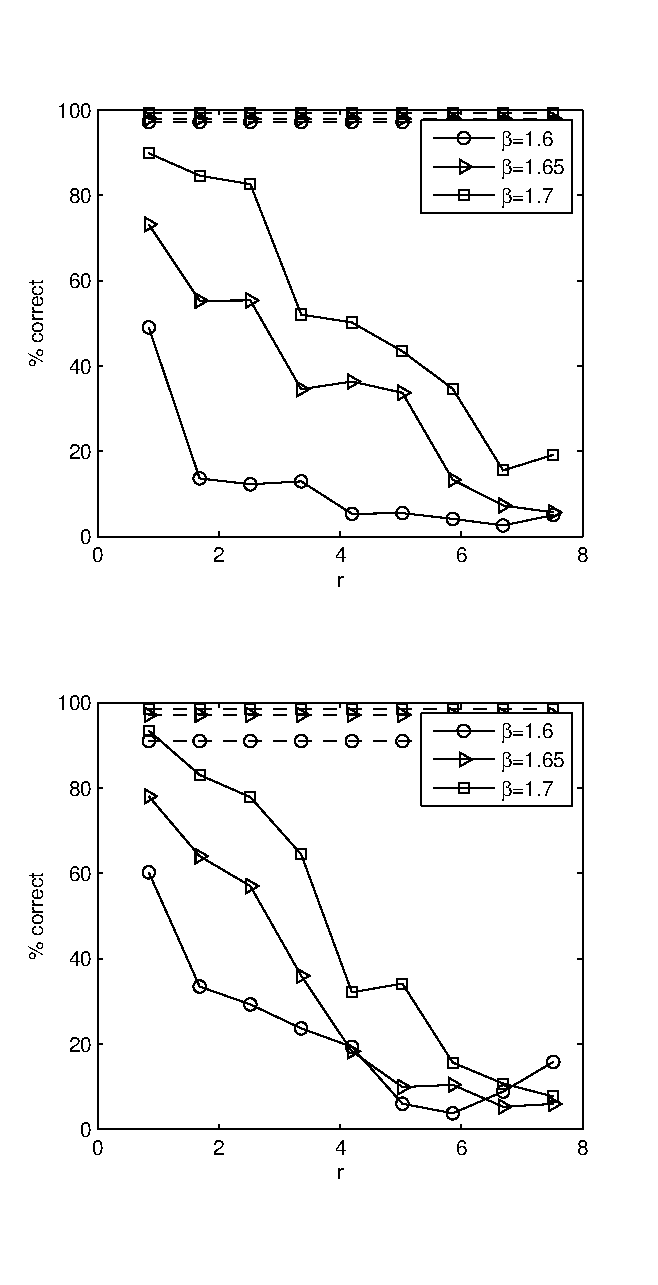
\includegraphics[width=6.5cm]{figures/newIndivSDRresults2.eps}
	\caption{Results for the two individuals from the signal detection experiment. The solid lines show the accuracy results for the target present trials, while the dashed lines shows accuracy for target absent.}
	\label{fig:newIndivSDRresults}
\end{figure}

The two subjects performed similarly and the mean target present performance is shown in Figure \ref{fig:meanRegression}. We will model this by using a simple multi-linear, with thresholding, model: 

\begin{equation}
f(\beta,r)= 4.09\beta-0.11r-5.97
$$\[ p(T|\beta,r) =  \left\{              \begin{array}{ll}                   f(\beta,r) & (f\geq0)\\                   0 & (f<0)              \end{array}       \right. \]$$
\label{linearregmodel}
\end{equation}
This regression model gives $R^2=0.934$. Note, the points $\beta=1.6,r=5.86,6.69,7.51$ were not including in the regression model. 

\begin{figure}
	\centering
		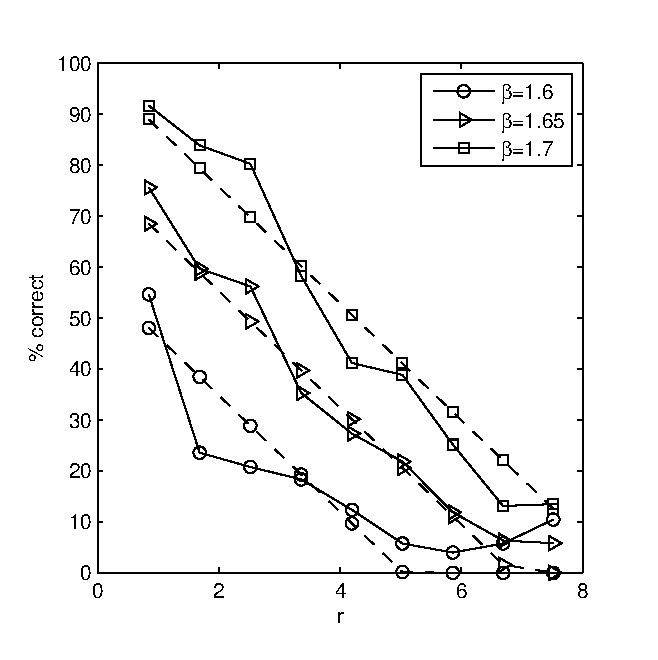
\includegraphics[width=6.5cm]{figures/meanRegression.eps}
	\caption{Solid lines show the inter-subject mean over $\beta$ and $r$ while the dashed line shows the best fit multi-linear regression.}
	\label{fig:meanRegression}
\end{figure}


\section{Simulation}
The simulation used the linear-regression detection model, based on the results of the signal detection experiment, together with data on human saccade distributions taken from previous work, to construct a stochastic model of saccade paths during visual search.

\subsection{Human Saccade Distributions}

In this section we will present a new analysis of data from the first of Clarke et al.'s [\citeyear{clarke2009}] visual search experiments. This experiment involved similar stimuli to those described above, although only 3 different target eccentricities were used. Seven observers completed the experiment and the task was simply to press a button on the keyboard once the target had been found. They were given unlimited time and an eye-tracker was used to monitor fixation locations. As the surface was made rougher (decreasing $\beta$ and increasing $\sigma_{RMS}$) a greater number of saccades were required to find the target. We will now carry out some further analysis of this data set. 

\par

The global saccade amplitude and direction distributions are shown in Figure \ref{fig:SaccadeStatistics} (top left and top right). As we can see, the saccade directions show the same horizontal bias as reported by \cite{gilchrist-harvey2006} and \cite{najemnik-geisler2008}. The saccade amplitude time series (Figure \ref{fig:SaccadeStatistics} (bottom left)) shows evidence for a coarse-to-fine search strategy, as reported by \cite{over2007}. 
\par
Figure \ref{fig:spatialsaccadestats} shows the distributions of saccade amplitude and directions according to the location of the starting fixation, in relation to the stimuli boundaries. For example, the largest saccade amplitudes appear to occur after a fixation is made near the corner of the stimuli early on in the search. Again, this agrees with the coarse-to-fine strategy described by Over et al. 
 

\begin{figure}
	\centering
		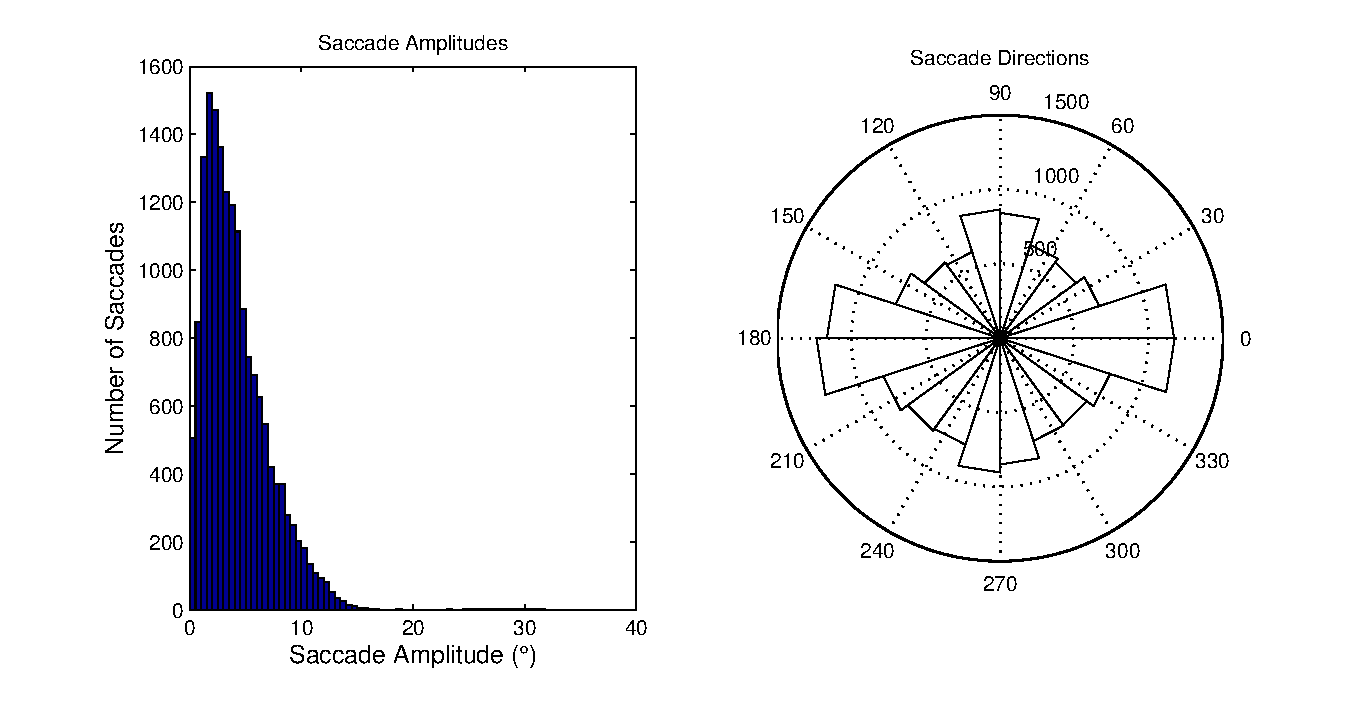
\includegraphics[width=7.5cm]{figures/SaccadeHistandRose.eps}
			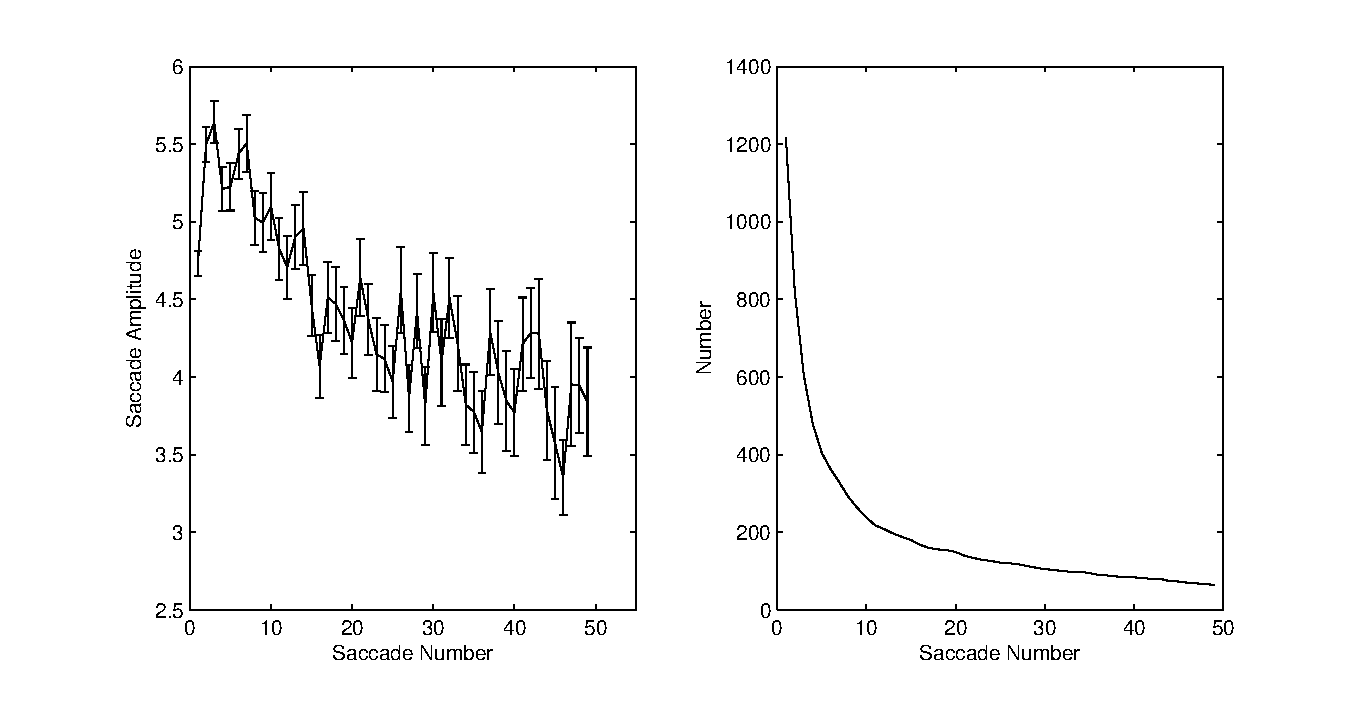
\includegraphics[width=7.5cm]{figures/SaccadeAmpOverTime.eps}
	\caption{(Top Left) Saccade amplitude histogram, (Top Right) Saccade direction rose plot, (Bottom Left) Saccade amplitude plotted against time, and (Bottom Right) The number of the fixations included in the analysis on the left.}
	\label{fig:SaccadeStatistics}
\end{figure}


\subsection{Algorithm}

\subsubsection{Inputs}
The model is given the size of the search area, $N$, the roughness of the surface $\beta$, and the target location (chosen randomly for a given eccentricity $r$). The initial fixation is set to the centre of the search area.

\subsubsection{Target Detection}
On each fixation the probability that the model detects the target is given by $p=f(\beta,r)$ where $f$ is the linear regression model described above. For each fixation we generate a random number $x\in[0,1]$ and check to see if $x\leq p$, in which case the model detects the target, makes a saccade to the target's location, and the search is terminated. If the model does not detect the target (i.e. $x>p$) then a random saccade is made to a new location. 

\subsubsection{Generating a Saccade}
In order to generate scan-paths we will use the empirical distributions of saccades (Figure \ref{fig:spatialsaccadestats}) as probability density functions. Since the amplitude distribution varies with the position of a saccade in the sequence made during a search trial we use separate empirical distributions for fixations $1\leq t\leq 5$, $6\leq t\leq 10$, $11\leq t \leq 15$ and $t>15$ (where $t$ is the fixation number). %The model is allowed to make a maximum of 200 fixations.

\begin{figure*}
	\centering
		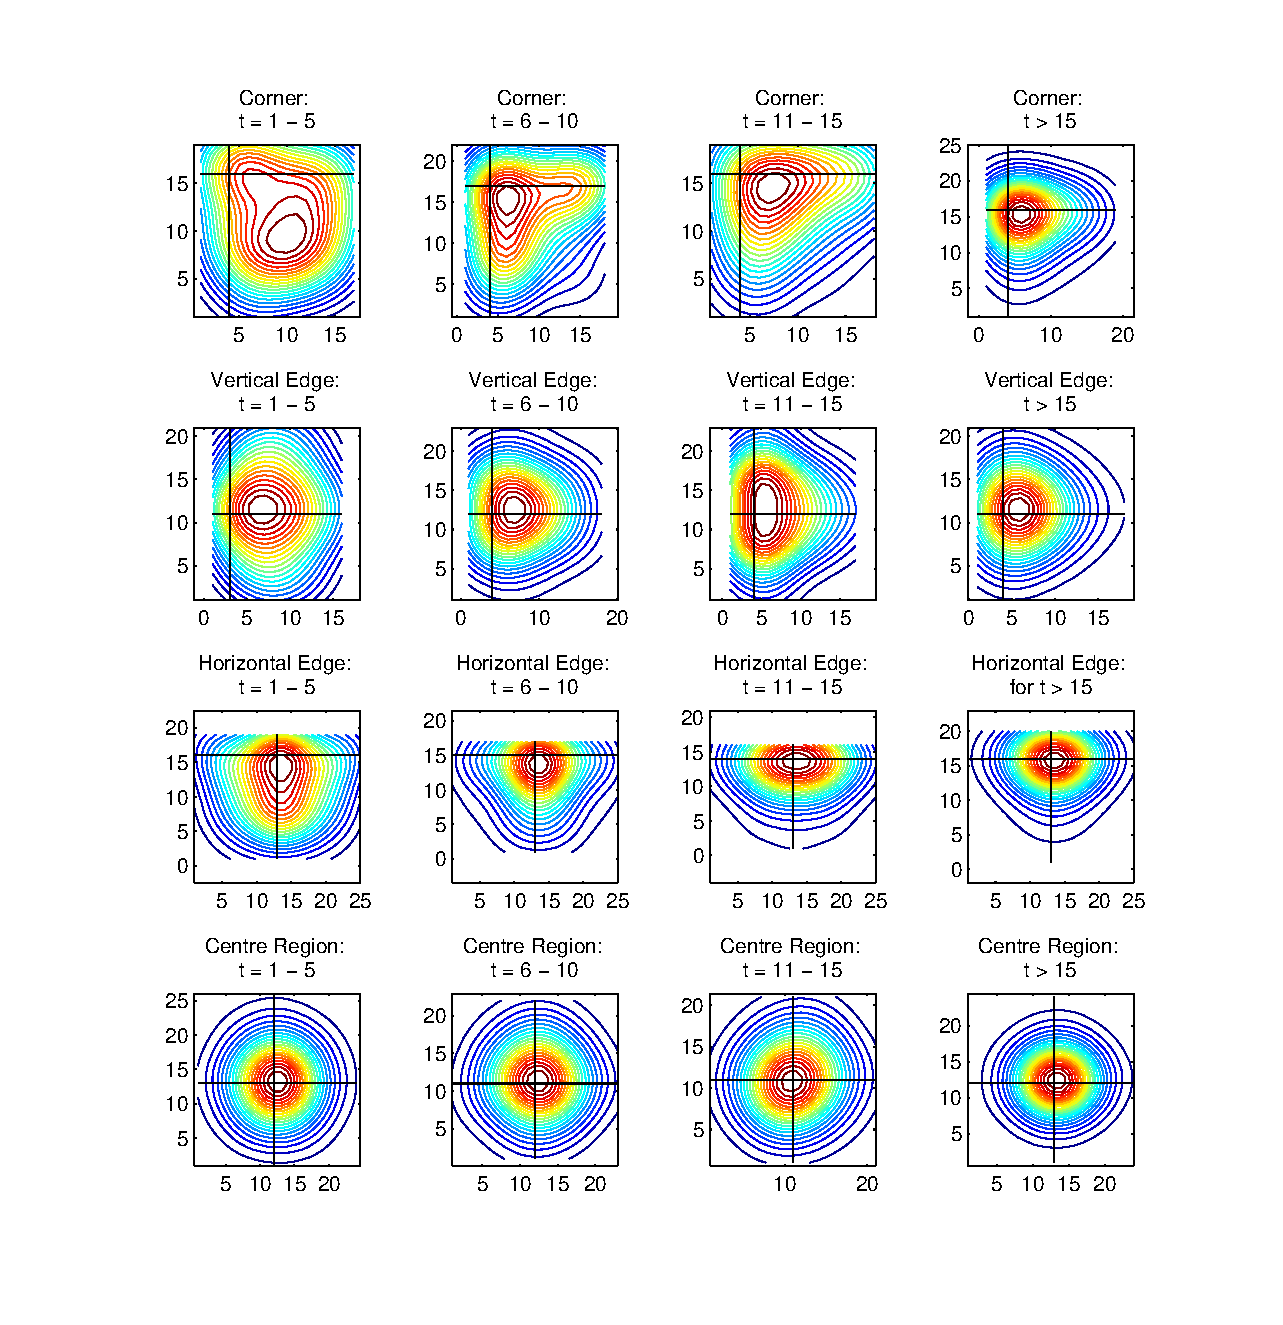
\includegraphics[width=14cm]{figures/saccadesbyposition2.eps}
		\caption{The effect of time and fixation location on saccades. These were created by dividing the search area into $5\times 5$ equally sized subregions. Horizontal and vertical axis of symmetry were assumed and used to combine information from the four corners regions. Similarly, the three remaining subregions along the left edge were reflected and combined with those along the right edge (similar for the top and bottom edges). Finally the nine central regions were grouped together.}
	\label{fig:spatialsaccadestats}
\end{figure*}


\subsubsection{Results}
Considering first the performance of the model in terms of the number of fixations required to find the target, we see that it performs in a similar way to the human observers in \cite{clarke2009} (Figure \ref{fig:Model_Human_numfix}). While the model slightly overestimates the number of saccades needed on easy surfaces, and underestimates the amount needed for harder surfaces, it remains within the 95\% confidence interval of the mean human observer.  

\par

\begin{figure}
	\centering		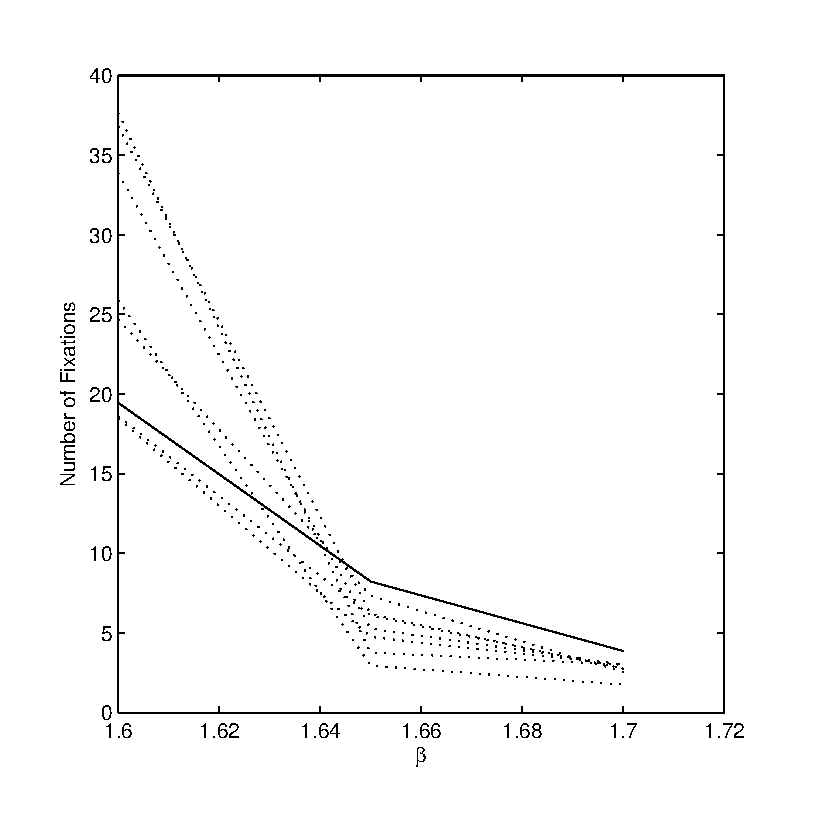
\includegraphics[width=7.5cm]{figures/Model_Human_numfix.eps}
		\caption{Comparison between human observers and the model. The top graph shows the performance, in terms of the number of fixations required to find the target, for each of the seven participants (dashed line), while the solid line shows the model's performance.}
	\label{fig:Model_Human_numfix}
\end{figure}
Next we compare how efficiently human observers and the model cover the search area during search. If human search has systematic properties we would expect the fixation locations to be approximately uniformly distributed: as there are no salient regions in the image apart from the target there is no reason to fixate any one area more than any other (except for a potential innate central fixation bias \citep{tatler2007}). The hotspot maps for the model and human observers are shown in Figure \ref{fig:hotspot}. For the human data, these included the first 30 fixations (excluding the initial fixation) from all trials in which at least 32 fixations were made (to minimise the effect of detecting the target. The model data was generated by simply running the model 105 times without the target detection component. The two hotspot maps were normalised. As we can see, the model appears to exhibit more of a central bias than the human data.

\begin{figure*}
	\centering
		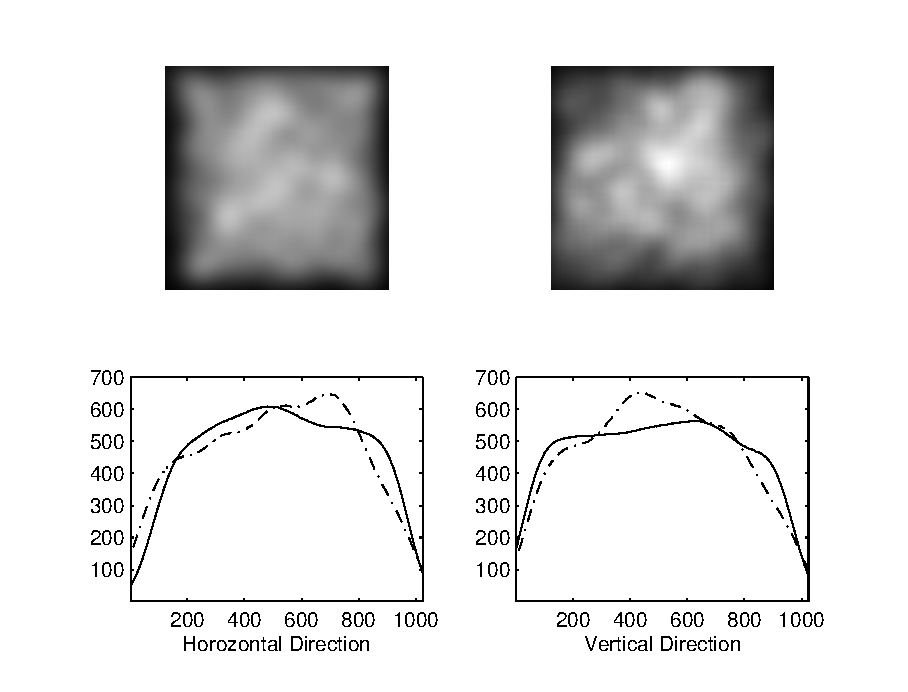
\includegraphics[width=14.9cm]{figures/hotspotcomparison.eps}
	\caption{(top left) Hotspot map of first 30 fixations over all trials (containing over 32 fixations) and observers. (top right) Hotspot map generated by the stochastic model. The stochastic model appears to be more biased towards the centre of the image. (bottom left/right) Density of fixations along the horizontal/vertical directions. Legend: (solid line) human observers (dashed line) stochastic model.}
	\label{fig:hotspot}
\end{figure*}

\par

Another way to compare how systematic human observers are is to look at the number of re-fixations. We have done this by checking each fixation to see if it is located within $30$pixels ($1/2^{\circ}$ of visual angle) of any of the previous three fixations. For each trial we computed the number of refixations per fixation. This number gives us an indication of how strong inhibition of return (IoR) is in the search task considered here and the results (see Figure \ref{fig:refixations}) show that humans appear to be no more systematic than the stochastic simulation. In fact, the model actually makes less re-fixations per fixation on the harder trials.

\begin{figure}
	\centering
		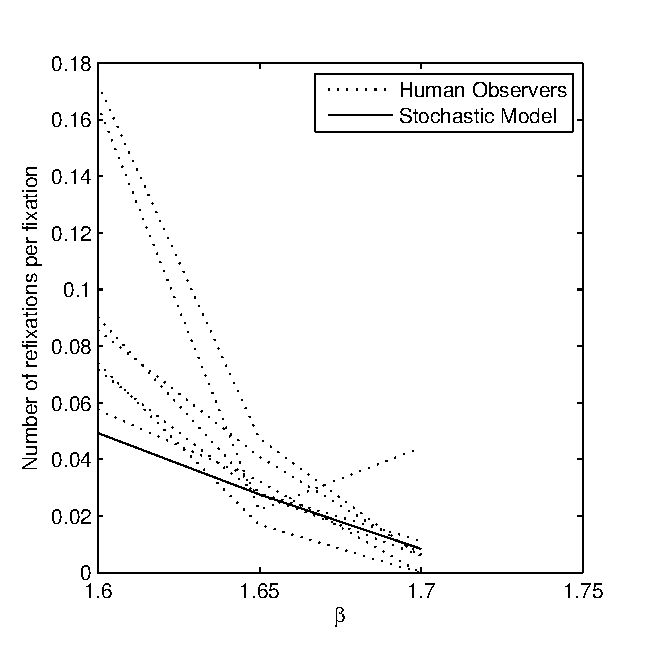
\includegraphics[width=7.5cm]{figures/refixations.eps}
	\caption{Number of times a saccade is directed to the location of one of the previous three fixations, divided by total number of fixations for that trial.}
	\label{fig:refixations}
\end{figure}

\par

Finally, we will use the Voronoi method proposed by \cite{over2006} to compare the distribution of saccades from the human and model. This method allows us to study the uniformity of fixation density and involves computing the bounded Voronoi cells \citep{voronoi1907} for a set of fixation coordinates and looking at the distribution of cell areas. Some examples of Voronoi diagrams can be seen in Figure \ref{fig:VoronoiExamples}. However, instead of looking at the skewness and fitting curves to the distribution of cell areas as Over et al. did, we will look at how the cells change over time, as successive fixations are made. A simple way of doing this is to look at how the area of the largest cell changes with fixation number. If search is systematic then we would expect observers to direct fixations towards regions of the display area which they have not already attended to and the size of the largest cell will fall more steeply than for a stochastic search.
\par

\begin{figure*}
	\centering
	\subfigure[Human Observer]{
		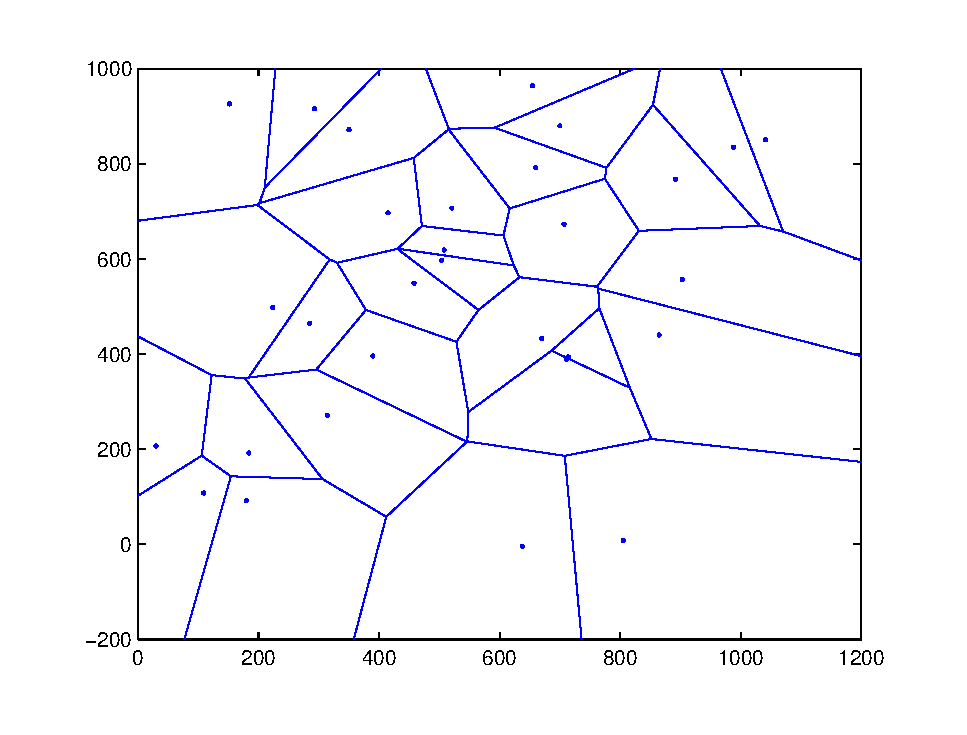
\includegraphics[width=7cm]{figures/Voronoi_new_human1.eps}}
		\subfigure[Human Observer]{
		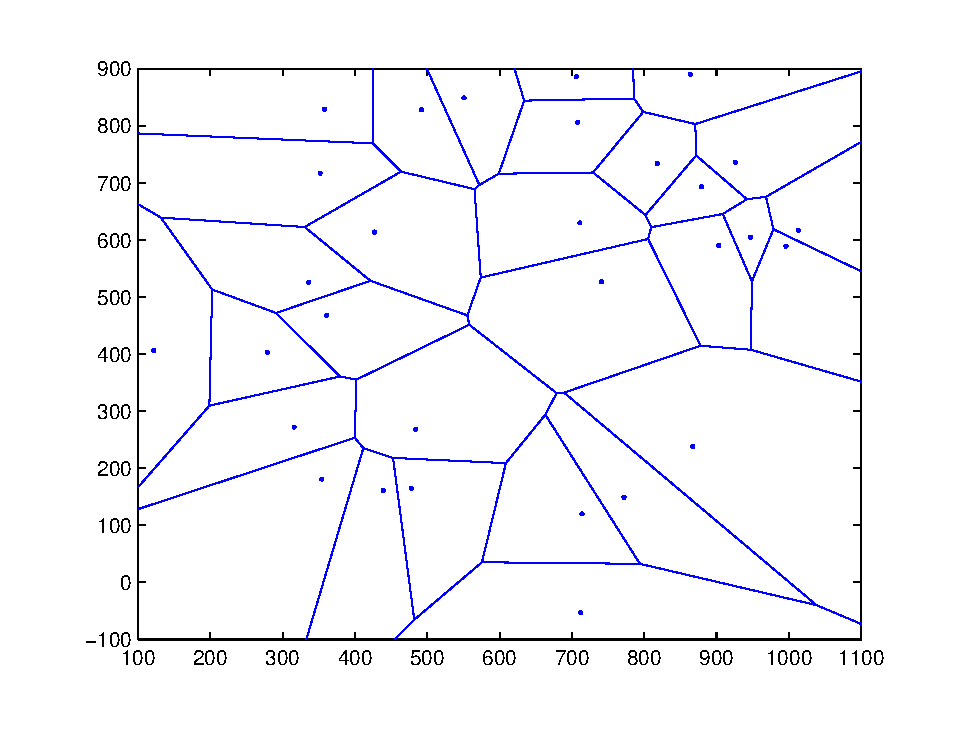
\includegraphics[width=7cm]{figures/Voronoi_new_human2.eps}}
			\subfigure[Model ]{
		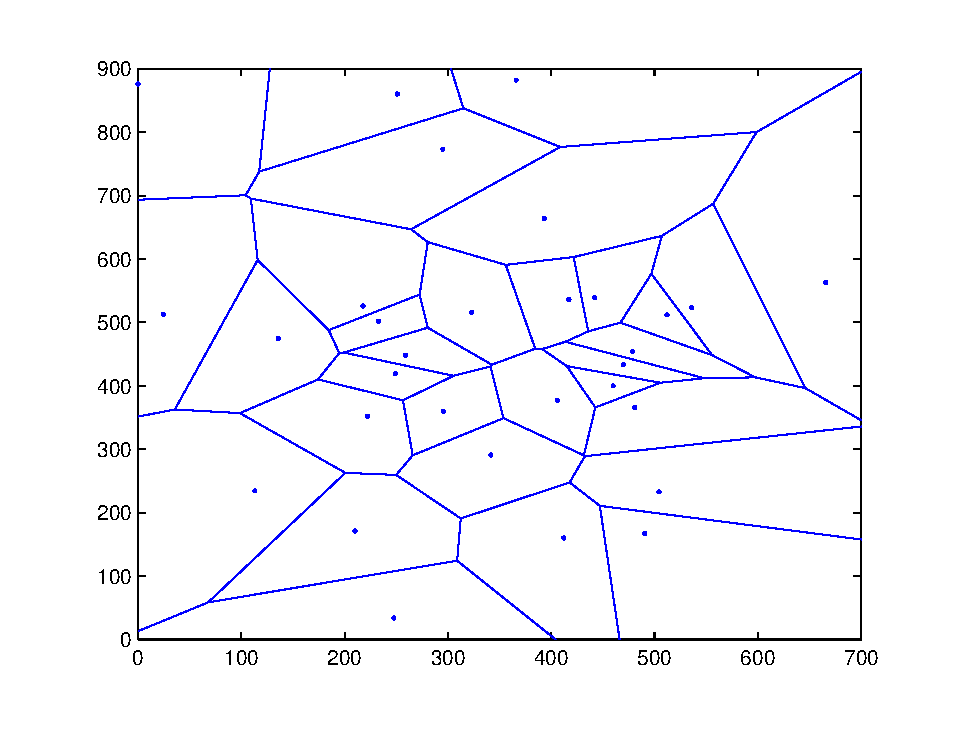
\includegraphics[width=7cm]{figures/Voronoi_new_model1.eps}}
		\subfigure[Model]{
		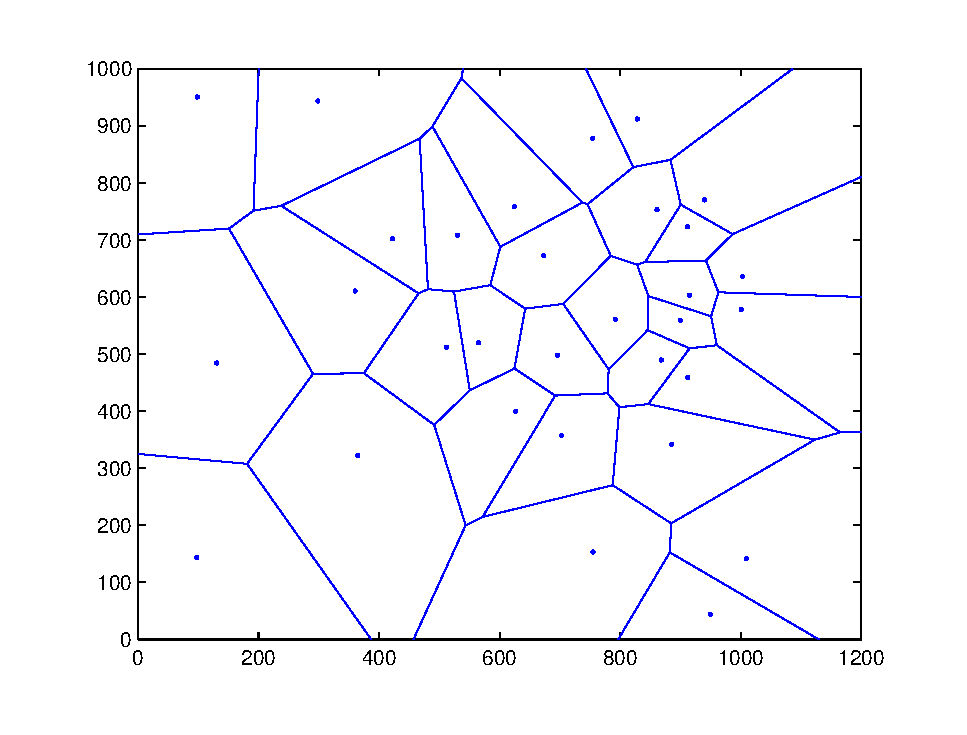
\includegraphics[width=7cm]{figures/Voronoi_new_model2.eps}}
		\caption{Examples of Voronoi plots from both the human observers and the stochastic model.}
	\label{fig:VoronoiExamples}
\end{figure*}


For each fixation $f_t$, ($t=1,\ldots,n-2$, where $n$ is the number of fixations in the trial), the Voronoi cells for fixations $f_1,\ldots,f_t$, are created and the the area of the largest cell, $A_t$ , is computed. The mean $A_t$, over all trials, is shown in Figure \ref{fig:VoronoiTime} (left). As we can see, the human observers outperform the stochastic simulation and the size of the largest Voronoi cell decreases rapidly durng the first 5 fixations. However if we look at the speed at which the observers reduce the size of the cell ($A_t-A_{t+1}$) we see that after the initial five fixations the stochastic simulation matches human performance (Figure \ref{fig:VoronoiTime} (right)).

\par

\begin{figure*}
	\centering
		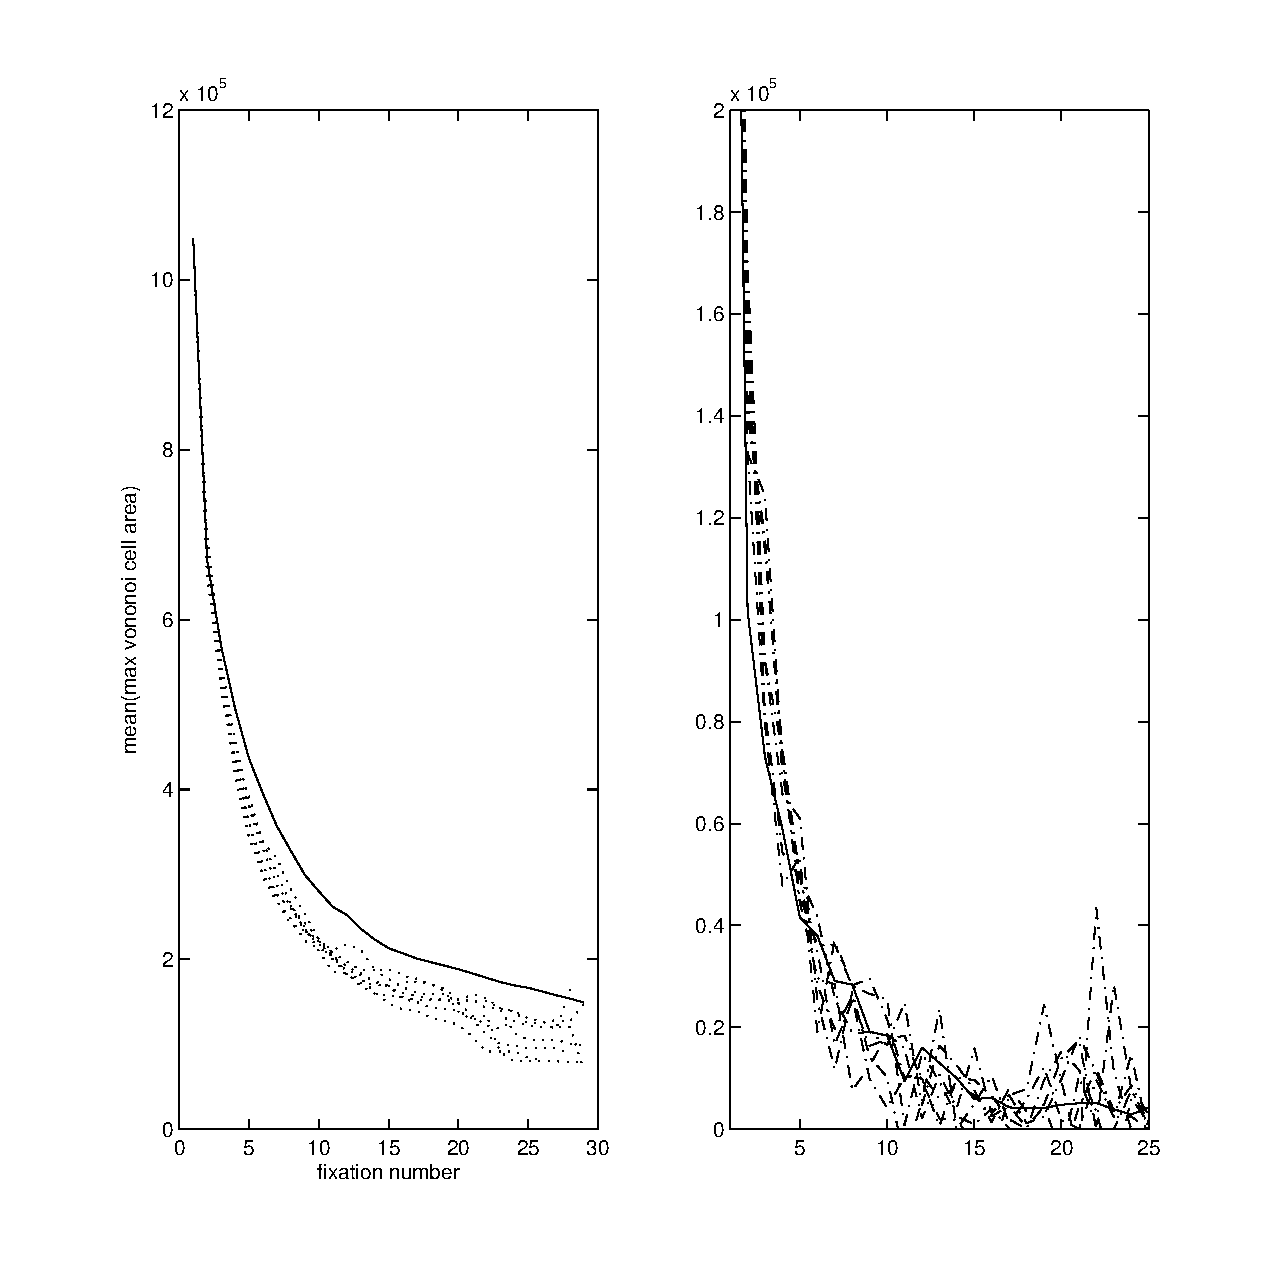
\includegraphics[width=14cm]{figures/VoronoiTime.eps}
	\caption{(left) How the maximum Voronoi cell area changes with time. Dotted lines show the seven human observers while the solid line shows the stochastic model. (right) This shows the derivative of the graph on the left: a measure of how quickly the search area is covered.	he main difference between the model and human observers occurs in the first few fixations. After these inital fixations human observers appear to be no more systematic than the model.}
	\label{fig:VoronoiTime}
\end{figure*}

\section{General Discussion}

The results suggest that, for visual searches involving locating a target on an otherwise homogeneous surface texture, human behaviour can be modelled closely by a stochastic process. The random walk model finds the target in a similar number of fixations as a typical human observer and produces scan-paths that are spatially distributed in a similar way to human scan-paths. The random walk model also makes a similar number of re-fixations and, except for the initial few fixations, searches as efficiently as human observers. 
\par
However, this is not to say that our results challenge Guided Search: in fact the two models could quite easily work together. In fact, the model presented in this paper \itshape is \normalfont guided. When the target is salient against the textured background then the model is likely to make a saccade to that location. One could imagine that if there are several search items that could potentially be the target, as there are in most typical visual search experiments, that a random walk model could be used to choose which item should be fixated next. Also, although our model did not need any form of memory or inhibiton of return, we do not mean to suggest that there is no inhibition of return in any form of human search. Indeed, as our stimuli contain no search objects, any IoR process would have to be operating with respect to spatial coordinates defined with respect to the stimulus boundaries, rather than being applied to discrete search objects. However, as we can see from Figure \ref{fig:refixations} human observers do not appear to re-fixate recently fixation regions any more or less than we would expect a stochastic, memory-less process to. Further research and experiments would be needed to characterise this behaviour more thoroughly. 
\par
This is a somewhat surprising result given that \cite{najemnik-geisler2008} have shown that human observers appear to be near optimal in their search strategy. Najemnik and Geisler also compared the spatial distributions of the fixations chosen by their ideal observer, a MAP model, and human subjects, and found that both human subjects and the ideal observer show a clear preference for fixation on small regions above and below the centre of the image. However, there is no evidence for this distribution in our data, which show no preferences for fixating any particular regions (see Figure \ref{fig:hotspot}). 

\par

There have been a series of papers using Classification Images to investigate guidance in a search task involving targets embedded in $1/f$-noise \citep{rajashekar2002, rajashekar2006, tavassoli2009}. This involves recording all the fixation locations and computing the mean region that is fixated on. For a search task involving a geometric shape embedd in $1/f$ noise, these classification images have been shown to resemble the target which is being searched for. However theses results do not appear to hold when the analysis methods are applied to the data from \cite{clarke2009}. The classification images obtained from the seven observers are shown in Figure \ref{fig:CIresults}. This could be because either guidance does not play a significant role with these stimuli or, due to the the small size of the target, there is a larger degree of variance in fixation placement with respect to the intended point of interest. This means that even if the observers were directing their attention to regions of the surface that resembled the target, they would be unlikely to be visible in the classification images. 

It could be that the target is too small when compared to the background and does not show up due to spatial uncertainties (need a better way of saying this). 

\begin{figure*}
	\centering
		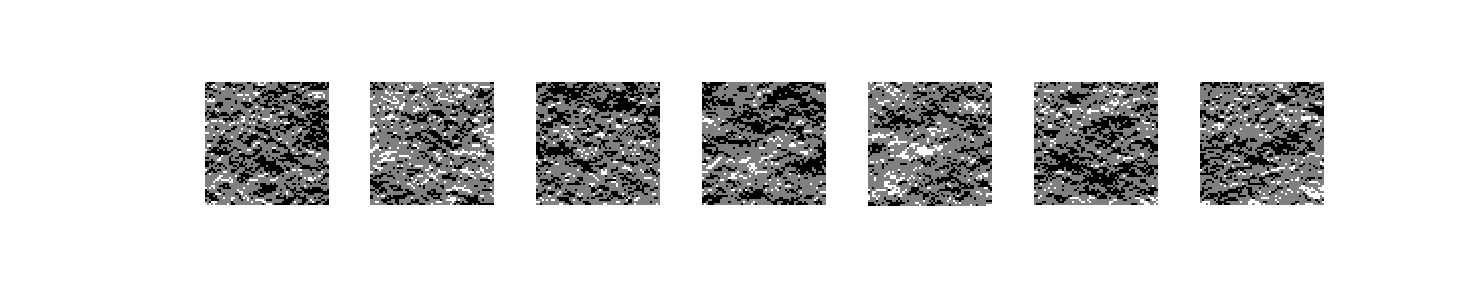
\includegraphics[width=14cm]{figures/CIresults.eps}
	\caption{Classification Images obtained for each of the seven observers in the first visual search experiment in \cite{clarke2009}}
	\label{fig:CIresults}
\end{figure*}

\subsection{Conclusions}
As stated above, a complete, computational visual search model should possess two parts: a feature extraction front end and a search strategy. The aim of this paper was to explore to what extent a search strategy based on a random walk could account for human performance. Previously implemented search strategies have generally worked in a serial manner, checking items one at a time, with some form of imperfect memory \citep{melloy2006, rutishauser-koch2007}. One search model that makes use of parallel target detection over a serial sequence of fixations is the Ideal Observer. One problem with this approach is that it assumes that the target will be located at one of a predefined independent finite number of potential target locations. Unfortunately, this assumption breaks down when image processing techniques are used, as the activation at any pixel is likely to be correlated with its neighbours. Hence we have explored an alternative explanation of human search strategies: a random walk. While the use of a random walk to explain patterns of fixations is not new \citep{greene2008, aks2002, morawski1980}, our model is unlike earlier ones in being strongly based on empirical data. We find that a random walk behaves in a similar way to human observers, both in terms of the number of saccades required to find the target, and the spatial distribution of fixations. 
\par
Our results here suggest that inhibition of return; integration of information across fixations, and more general memory based processes do not have a large role to play in at least one type of search task (search for an inconspicuous target on a continuously textured surface). Future testing of models of visual search should consider not only possible differences between search strategies on different types of stimuli, but also variation between observers in their strategies. It may be possible to obtain evidence for more than one model of search strategy depending on the observers tested.

\appendix
\section{Appendix: LNL model comparison}
\label{appendix:LNL}
In our previous work we have applied an LNL-based model to the problem of modelling search for a target on a rough surface (Clarke, et al., 2009). A bank of Gabor filters was applied to the input image and then passed through a non-linearity. This nonlinear processing strengthened the signal of filter response maps containing a small number of strong local maxima (as opposed to maps which contained a large number of local maxima). Finally these feature maps were passed through a 2nd order linear filter (local energy pooling) before being summed together to give an activation map. This activation map was then passed to a simple saccade selection algorithm. For each fixation an exponential distance dependant fall-off was applied to the activation map along with a simple inhibition of return process. The model would then randomly select one of the n (=3) largest local maxima as its saccade target.
\par
While the algorithm succeeded in modelling human performance (in terms of the number of saccades required to find the target), it did not account for the selection of individual fixation points on each saccade, in trials where more than one or two saccades were required to find the target. There was no apparent relationship between human fixation locations and (non-target) local maxima in the activation map. While one possibility would be that the fall-off function is too strong, we can discard this suggestion as weakening the activation fall-off function would cause the model to diverge from human performance in terms of number of saccades to targets at high eccentricities. 
\par
To explore this further we compared saccade targets for the model with those chosen by human observers  in the experiment reported by \cite{clarke2009}. Over all observers, trials and fixations, 22\% of saccades were directed to within $1^{\circ}$ of one of the three saccade targets considered by the model, and over 25\% fell more than $4.3^{\circ}$  (equal to a quarter of the display's length) away from the nearest point considered by the model.  The LNL model is therefore able to predict the locations of only a small proportion of non-target fixations during visual search. Furthermore, most of the successful cases can be accounted for by chance. Let us assume (a) that all model and human saccades are no more than $r$ in amplitude; and (b) 	the three potential fixations considered by the model are separated from each other by at least $2^{\circ}$
\par
Then the fixations will occur somewhere within an circle with area $A=\pi r^2$. Therefore the probability of the human saccade landing within $1^{\circ}$ of one of the model's saccades is $p=3\pi/A=3/r^2$. If we take $r=4^{\circ}$ (over half of the human saccades are under $4^{\circ}$ in amplitude) then we would expect human observers to fixate within $1^{\circ}$ of one of the fixation locations considered by the model 19\% of the time, which is close to the 22\% we obtained from the empirical comparison. 
\par
The above analysis suggests that the LNL model, while offering a good prediction of the difficulty of the search task, does not succeed in modelling saccade selections any better than if it did not possess an activation map.

\section{Appendix: Texture Synthesis}
\label{appendix:synthesis}

For the experiments in this paper a very simple model referred to as $1/f^{\beta}$-noise will be used. We can represent a surface by an $n\times n$ matrix $h$. This matrix is referred to as a height map and for any $(x, y)\in\{Z\times Z | 0 < x, y < n\}$,$ h(x, y) = z$ gives us the height of the surface. The $1/f^{\beta}$ noise has only two parameters: the frequency roll-off, $\beta$, and the RMS-roughness, $\sigma_{RMS}$. The RMS-roughness is the standard deviation of the surface's height map and acts as a scaling factor in the $z$-axis. The roll off factor $\beta$ controls the amount of high frequency information in the surface: increasing $\beta$causes the high frequencies to drop off more quickly, so the texture appears smoother \citep{padilla2008}. Note that we use $\beta$ here to denote the roll-off of the magnitude of the inverse discrete Fourier transform of the height map. The same term and symbol also sometimes refers to the roll off factor in the power spectrum of an image. See \cite{chantler2005} for a model relating these two parameters. 
\par
The surface is generated in the Fourier domain with the magnitude spectrum given by:
\begin{equation}
S(u,v)=\frac{k}{\sqrt{u^2+v^2}}
\end{equation}
where $k$ is the scaling factor required to give the desired $\sigma_{RMS}$. The phase spectrum is randomised and by using different values to seed the random number generator we can create many different surfaces with the same properties. Taking the inverse discrete Fourier transform of the magnitude and phase spectra gives us our height map $h$.

\par
The two dimensional height map that represents our surface texture is then rendered to
generate an image of the surface under specified illumination. This stage is important, as a surface can have drastically different appearances under different light conditions \citep{chantler1995}. We will use one of the simplest models, known as Lambert's Cosine Law. This treats the surface as a perfectly diffuse reflector, i.e. it reflects the same amount of light in all directions. It is easily modelled by the dot product:
\begin{equation}
i(x,y) = \lambda . \rho (x,y) \underline{n}(x,y) \underline{l}
\end{equation}

where $i$ is the image we are creating, $\underline{n}$ is the unit surface normal to
the height map and $\underline{l}$ is the unit illumination vector. The albedo, $\rho$, determines how much light is reflected by the surface. The strength of the source light is denoted by $k$. The surface normal $\underline{n}$ is estimated by:

\begin{equation}
p(x,y) = h(x,y)-h(x-1,y) \ \  \  \  q(x,y)=h(x,y)-h(x,y-1)
\end{equation}
\begin{equation}
\underline{n} = \frac{1}{\sqrt{1+p^2+q^2}}[p,q,1]^T
\end{equation} 
 
Self shadowing occurs when $i(x,y)<.0$ i.e. the surface is orientated such that its normal makes an obtuse angle with the illumination vector. Self shadowing is implemented by setting all negative values to 0. Cast shadows are not implemented in this model. The illumination conditions will be kept constant throughout this paper with elevation $= 60^{\circ}$ ,azimuth = $= 90^{\circ}$ and the strength of the source light being set at 150 $cd/m^2$. The albedo value will be kept constant at 0.8 throughout all the experiments, which is approximately the value of matte white paint.
\par
To use rendered surfaces in visual search experiments, we need to choose a target. Rather than using a target with an artificial appearance, we create an anomaly in the surface texture, in the form of a small pothole in the surface. We create these targets by subtracting the lower half of a small three dimensional ellipsoid from the surface. Our ellipsoid defect is defined by
\begin{equation}
\frac{x^2}{a^2}+\frac{y^2}{b^2}+\frac{z^2}{c^2}=1
\end{equation}
To make the indent appear more realistic it is convolved with a two dimensional smoothing filter to soften the hard vertical edges.




%%%%%%%%%%%%%%%%%%%%%%%%%%%%%%%%%%%%%%%%%%%%%%%%%%%%%%%%%%%%%
%% BIBLIOGRAPHY AND OTHER LISTS
%%%%%%%%%%%%%%%%%%%%%%%%%%%%%%%%%%%%%%%%%%%%%%%%%%%%%%%%%%%%%
%% A small distance to the other stuff in the table of contents (toc)
%\addtocontents{toc}{\protect\vspace*{\baselineskip}}

\bibliographystyle{plainnat}
\bibliography{literature}
%% The List of Figures
\clearpage
\addcontentsline{toc}{chapter}{List of Figures}
\listoffigures

%% The List of Tables
%\clearpage
%\addcontentsline{toc}{chapter}{List of Tables}
%\listoftables


%%%%%%%%%%%%%%%%%%%%%%%%%%%%%%%%%%%%%%%%%%%%%%%%%%%%%%%%%%%%%
%% APPENDICES
%%%%%%%%%%%%%%%%%%%%%%%%%%%%%%%%%%%%%%%%%%%%%%%%%%%%%%%%%%%%%
\appendix
%% ==> Write your text here or include other files.

%\input{FileName} %You need a file 'FileName.tex' for this.


\end{document}

